\documentclass[a4paper,titlepage]{report}

\usepackage{geometry}
\usepackage{graphicx}
\usepackage{amssymb}
\usepackage{mathtools} 

\geometry{
  includeheadfoot,
  margin=2.54cm
}

\begin{document}

\begin{titlepage}

\begin{center}
 
\Large\textbf{Department of Physics and Astronomy\\
University of Heidelberg}

%change back when submitting
%\vspace{18cm}

\vspace{16cm}

\normalsize
Bachelor Thesis in Physics\\
submitted by\\
\vspace{0.5cm}
\Large\textbf{Maximilian Argus}\\
\normalsize
\vspace{0.5cm}

born in Hamburg, Germany\\
\vspace{0.5cm}
\Large\textbf{1990}
\normalsize

\newpage




\Large\textbf{Electric Field Optimization of a Rydberg Atom Experiment}

\vspace{18cm}

\normalsize
This Bachelor Thesis has been carried out by Maximilian Argus at the\\
Physikalisches Institute in Heidelberg\\
under the supervision of\\
Prof. Dr. Matthias Weidem\"uller

\vfill
\end{center}

\end{titlepage}


\begin{abstract}
Modern experiments with ultracold Rydberg atoms with application to many body physics and quantum information science, demand a  high level of experimental sophistication to precisely control experimental parameters like external electric fields, as Rydberg atoms are very  polarizable. In the experiment this is achieved by (a structure hosting) >10 individually controllable electrodes. However, the task of finding the optimal control voltages for these is complicated by incomplete knowledge of the charge distributions, including possible patch fields (making it particularly time consuming). To overcome this challenge we have applied evolutionary algorithms, a group of powerful search heuristics, to optimize the overall performance of our experiment. With particular focus on electric field control we asses the performance of several algorithms, on competing requirements of noise robustness and fast convergence, in solving two problems: cancellation of electric fields and and optimum guiding of field ionized Rydberg atoms to a MCP detector. Additionally Foreseeable applications to controlling quantum state evolution and engineering strongly correlated many body systems of interacting Rydberg atoms will be considered. 

\end{abstract}



\section*{Introduction}
Introduction introduction introduction

\tableofcontents

\chapter{Concept}

The aim of this thesis is the application of optimization methods to a Rydberg atom experiment. In the course of making one measurement several steps have to be completed sequentially. These start with collecting Rubidium atoms into a MOT, pre-cooling then and then loading them into a diplote trap where they are exited into Rydberg atoms. After this has been done the atoms can be imaged by a camera system. These steps form a cycle that is repeated every few seconds with variation of parameters in order to make measurements of the change in beahaviour of the Rydberga atoms dependends on the varied parameters. While many properties of the experimental setup are physically fixed, such as the position of the lasers, a relativley large number (77) that can be controlled by the software controlling the experiment, such as the timing of activating these lasers. The aim of this project is to add information feedback to this cycle, so that the experiment can choose new experimental parameters based the results of previous evaluations. The scematic for this is shown in figure 1.1

\begin{figure}[htb]
\centering
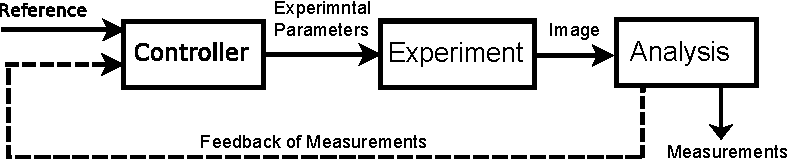
\includegraphics{Images/Feedback.pdf}
\caption{Information Feedback}
\label{fig: Information Feedback}
\end{figure}


Due to the discrete nature of experimental cycle evaluations and the large number of paramters as well as considerable measurement noise an opimization approach was choosen that generates and evaluates new experimental parameters. Using one can define the goal of the optimization as a function of several of the measurement results calculated by the analysis step.

Of particular interest is the control of experimental electrodes sourrounding the Rydberg atoms. One of the experimental goal is creating minimal electric fields as the predictions that are made assume a field-free environment. Additionaly it is important to generate a homogeneous filed as this prevents position dependent energies. When working with Rydberg atoms one mostly want to increase the principle quantum number $n$ in order to scale with it the physical effects one is trying to measure, however the polarizability of Rydberga atoms scales with $n^7$ requiring fine control over the electric field if one wants to work with larger Rydberg atoms.



\chapter{Theoretical Background}

\chapter{Optimization}

\section{Mathematical Formulation}
A $n$ dimensional real value optimization problem can be stated in the form
\[ min f(\mathbf{x})  \]
for
\[ f: S \rightarrow  \mathbb{R} \]
where
\[ \mathbf{x} \in S  \subseteq \mathbb{R}^n \]

\noindent
A point $\mathbf{x}^* \in D$ is a global minimum if  $ f(\mathbf{x}^*) \leq f(\mathbf{x}^*)  \forall  \mathbf{x} \in S$

\noindent
A point $\mathbf{x}^* \in D$ is a local minimum if  in the surrounding  $ U \subseteq S$ of  $\mathbf{x}^*$ it holds that $f(\mathbf{x}^*)  \leq f(\mathbf{x})  \forall  \mathbf{x} \in U$


\section{Background: Why look at multiple algorithms?}
There are a large number of optimization algorithms that have been developed in order to solve different problems. The key to applying optimization algorithms then is to find one suitable to solving kind of problems one is working with. Abstractley this is the converse to the No Free Lunch Theorem which states that the average performance of an optimizationa algorithms, when applied to the set of all optimization problems,  does not outperforom any other optimization algorithm or random walk. An algorithm is thus only, compartivley, suitable if it is able to utilize some form of problem specific information coupling the choice of algorithm to the problem at hand.

Due to the kind of problems to which optimization is to be applied to only the subset of Monte Carlo probablistic global optimization algorithms will be considered. These algorithms sacrifice both evaluating the entire search space and the necessity of evaluating the function exactly in favour of a shorter runtime. In these algorithms the choice of which candidates to evaluate is made by a heuristic which makes an induction based on previous evaluations. It is in this heuristic that is represents the problem specific information of the optimization algorithm.


\section{Evolutionary Algorithms}

Evolutionary Computation repersents a subset of heuristic based approaches in which a set of possible solution candidates is maintained which the algorithm tries to refine over a number of generations. In the following sections we will introduce the differnt categories of algorithms used as well as the specific implementations of algorithms from these categories. 


\section{Genetic Algorithms}

First we start with a simple genetic algorithm that will serve as a template for the algorithms to follow. In this algorithm we will encounter the common components of evolutionary algorithms, which are seen in the following block diagram. 


\begin{figure}[htb]
\centering
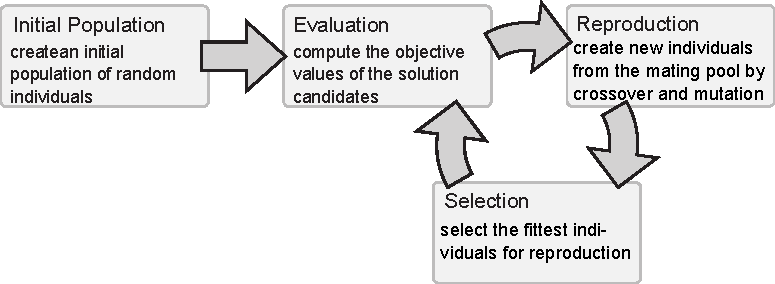
\includegraphics{Images/evolution_v2.pdf}
\caption{Block diagram of an Optimization Algorithm \cite{weise}}
\label{fig: genetic algorithms}
\end{figure}

\subsection{Generation}
In order to start an opimization process one needs an intial population, as optimization is usually done over a restriced search space, one tries to  choose an initial population of candidates one tries to sample the search space as even as possible. This decreases the chances of missing the location of the global minimum as well as avoids biasing the optimization to any particular region. This is usually achieved by using a uniform random distribution. An alternative is to use quasirandom sampling based on halton sequences which are more equidistributed. This reduces the chances of evaluating candidates that are very similiar at the cost of exploring the whole solution space.

\begin{figure}[htb]
\centering
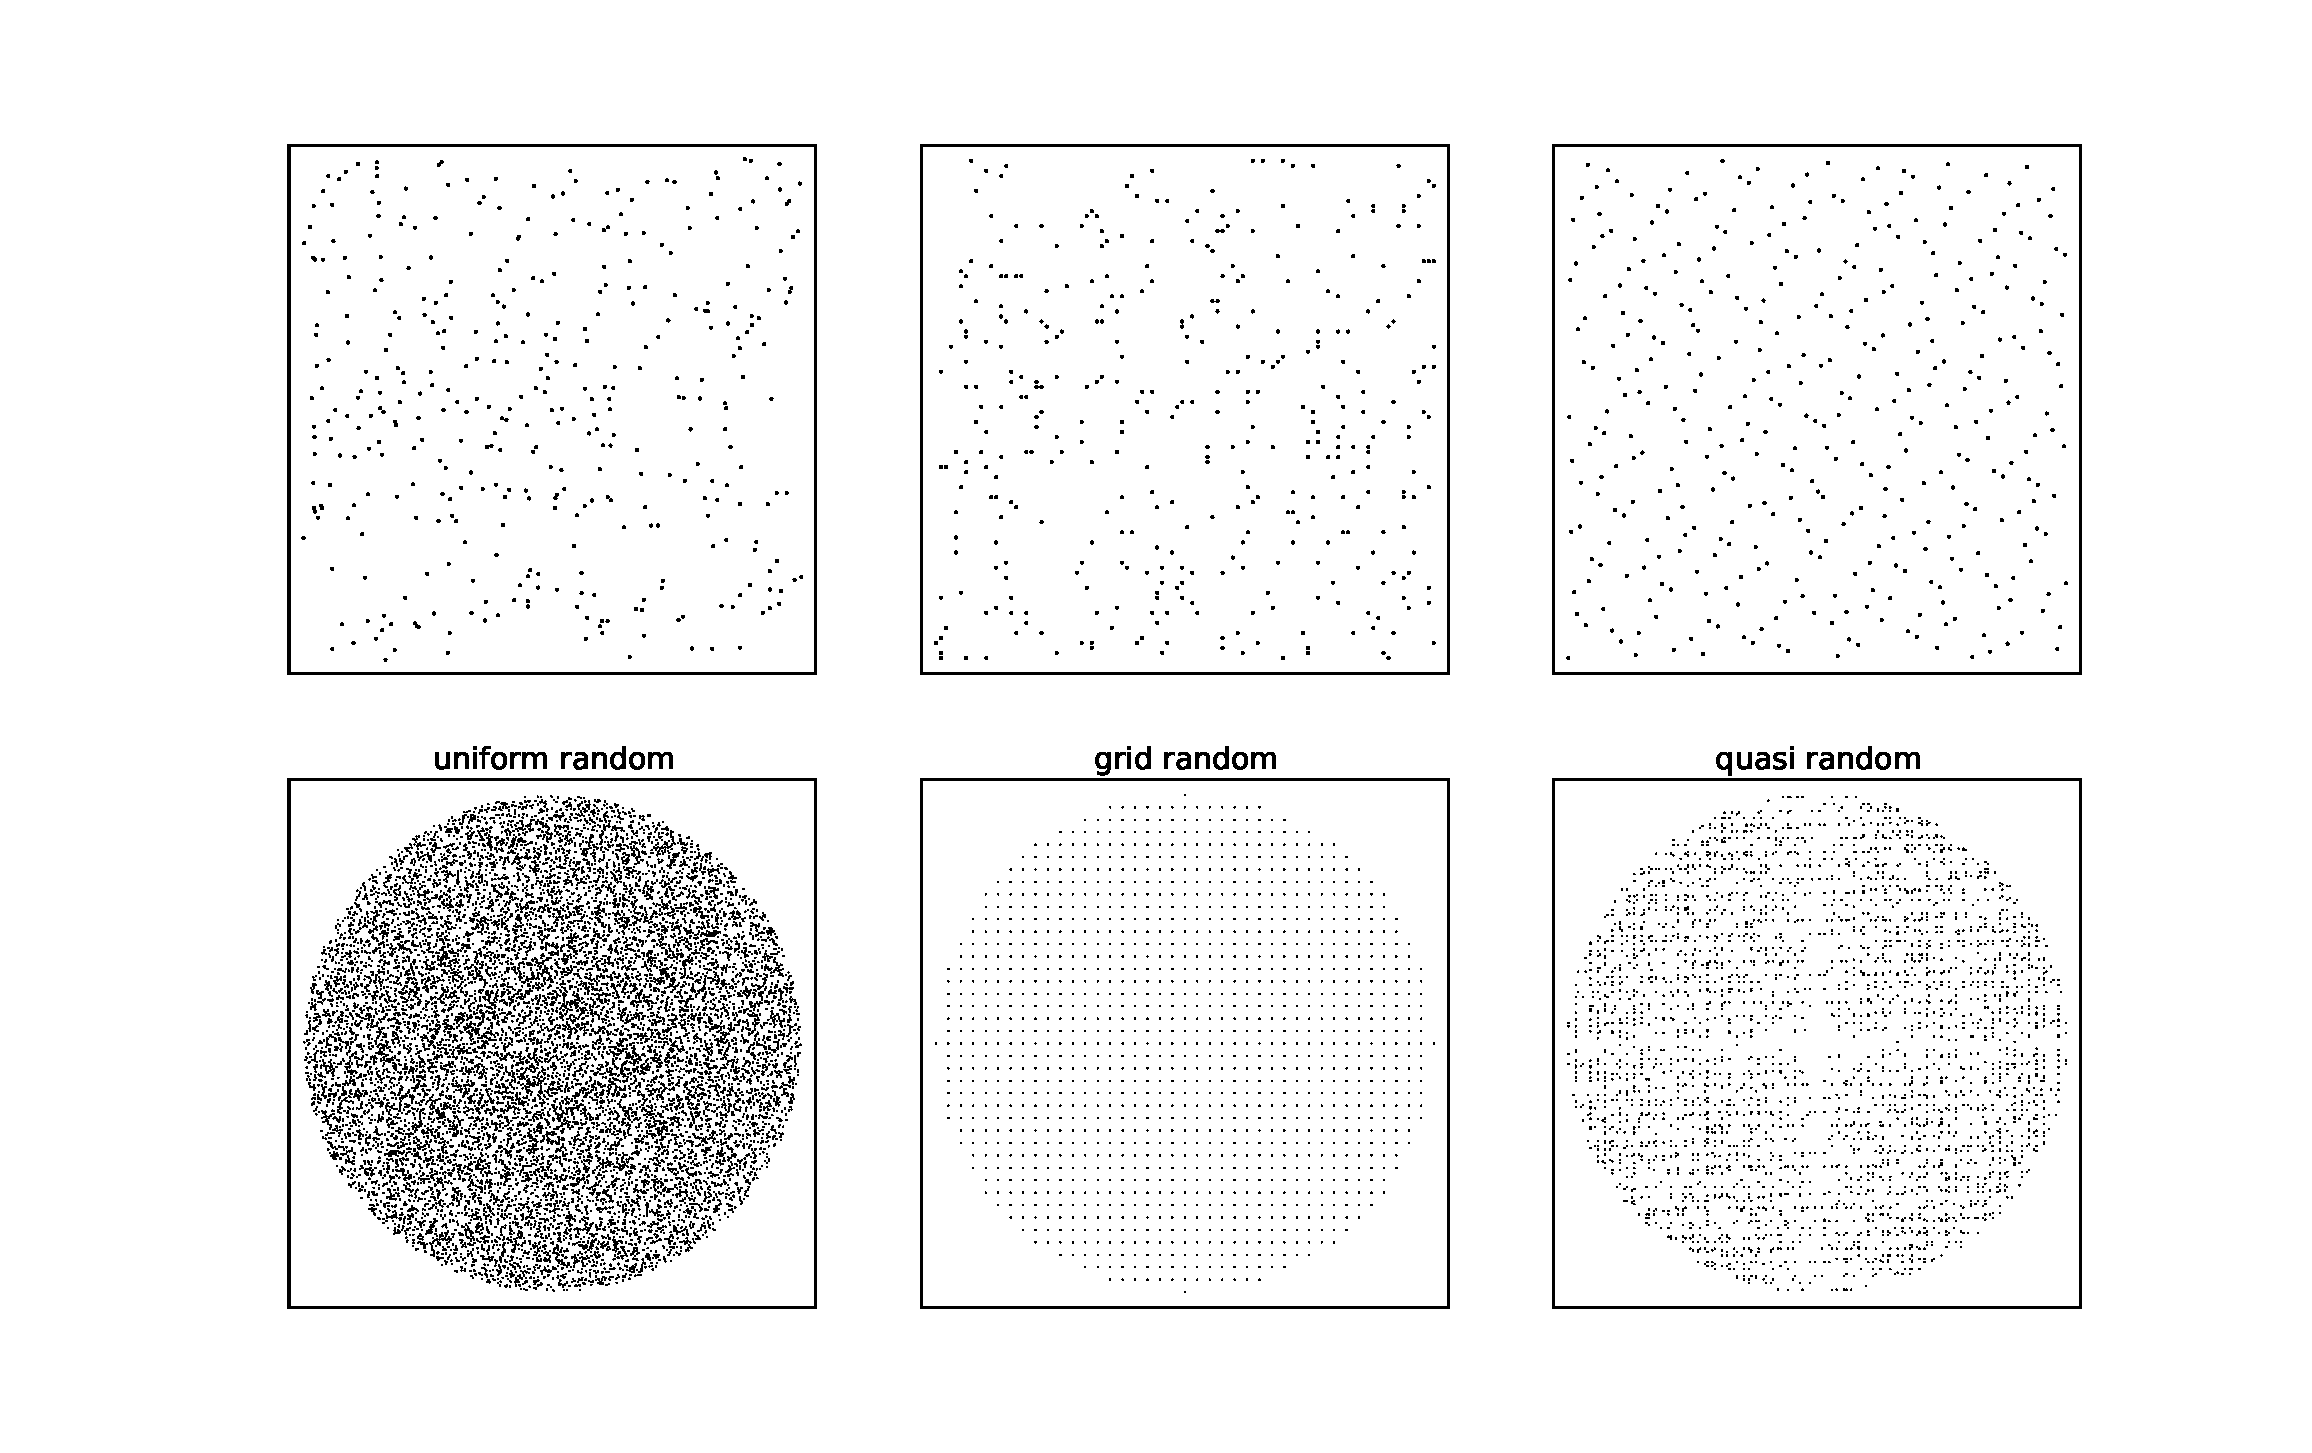
\includegraphics[width=16cm]{Images/sampling.png}
\caption{Three different sampling methods. The upper plot shows the similar looking positions sampled on a 1x1 square. The lower plot shows the relative distance of each point to all of its neighbours in a .2 radius. \cite{hayes} }
\label{fig: sampling}
\end{figure}

\subsection{Evaluation}
Following the initial population choice these candidates are evaluated. In our case this is the most time consuming part of the optimization process as it requires an completion of the experimental cycle, thus there is not a lot that can be done to optimize this step.

\subsection{Selection}

Once the population has been evaluated the better candidates need to be selected as parents of the following generation. The aim here is to have the choice of parents be influenced by the fitness but not doing this too strongly as it would decrease the diversity of the population.


\subsection{Variation}

Given two different parents one can create a child candidate by mixing the paramter vectors of the two parents. This process is called a crossover operation, the most basic of which is the one point crossover where every value up to a certain index is copied from one parent, and the following entries are copied from the other parent. Another way of varying a child  is through "mutation" that is performed by adding gaussian nosie to the element of a child vector.


\subsection{Exploration vs. Exploitation}

One of the treadeoffs inherint in global optimization is the choice between exploration and explotation. Exploration is the unbiased search for solution candidates in the whole search space whereas exploitation consists of trying to follow the lead of good solution candidates that have already been found. When the risk of an algorithm exploring too much is greatly increased runtime it is more likely to find the global optimum conversley an algorithm that exploits good solution candidates too strongly will follow inital leads and get stuck in a local minimum. There are a number of ways that this behaviour can be controled in during the selection and variation stages of an algorithm. The population size chosen also has a strong effect.


\section{Differential Evolution}

Differential evolution is an optimization algorithm belonging to the Evolution Strategy family of optimization algorithms developed by Storn and Price \cite{storn}. It destinguishes itself by a special kind of three parent "differential" crossover variation that follows the form:

\[ \mathbf{v}_{i} = \mathbf{x}_{j} + F \cdot ( \mathbf{x}_{k} -  \mathbf{x}_{l} ) \]

Here $j,k,l \in \{1,2,\dots,NP\} / \{i\}$ are random vextor indexes anf $F \in [0,2]$ is a weighting factor wich controls the weight of the differental varation. However this new vector is not used directly, a binomial crossover witht the intial vector $\mathbf{x_i}$ is performed, in which each element is chosen as the result of an independent binomial experiment.

\newcommand*{\bfrac}[2]{\genfrac{}{}{0pt}{}{#1}{#2}}

\[ \mathbf{x}'_{i,m} = \left\{ \bfrac{ \mathbf{v}_{i,m} \; \text{for}\; (r_m \le CR) \lor (r_i = j) }{ \mathbf{x}_{i,m} \;\text{for}\; (r_m > CR) \land (j \ne r_i) } \right. \]
\[ \forall m \in \{1,2,\dots,D\} \]

Here $r_i$ is a random integer index chosen once for each vector and $r_m \in [0,1]$ in a random number chosen once for each vector element. This results in at least one component of the new vector coming from the varied one. The resulting vector $\mathbf{x}'$ is then kept if it has a better fitness values than its predecessor $\mathbf{x}$.

Differential evolution algorithms exist in a number of different variations that are named using the notation

\[DE/x/y/x\]

x represnets the way in which the population should be varied. It can stand for "rand" or "best". With"rand" a randomly chosen vector is varied, as was previously explained and with "best" the best vector of the population is varied.

y is the number of difference vectors used, currently one.

z specifies the crossover scheme used, this can be "bin" for binomial crossover or "exp" for exponential crossover.

Using this notation the algorithm we have described would be represented by

\[DE/rand/1/bin\]



\section{Swarm Intelligence}

Particle swarm optimization was initially developed by Kennedy and Eberhart to model the beahviour of a flock of birds. It was then noticed that the model could could be applied to do black-box optimization. In this method each particle has a position $\mathbf{x}$ and a velocity $\mathbf{v}$. In each iteration of the optimization the velocity is computed by the formula:

\[ \mathbf{v} = \omega \mathbf{v} + \phi_p r_p (\mathbf{p} - \mathbf{x}) + \phi_g r_g (\mathbf{g} - \mathbf{x}) \]

Where the parameter $\omega \in \mathbb{R}$ is the inertia weight. $\mathbf{p}$ and $\mathbf{g}$ are the best positions discovered by the particle and the swarm respectivley. The attraction to these positions is controlled using the paramters $\phi_p, \phi_g$ and varied stochastically using $r_p,r_g = U(O,1)$. With each generation the velocity is applied to the position

\[\mathbf{x}' = \mathbf{x} + \mathbf{x} \mathbf{v} \]

This results in the swarm ideally converging on the global optimum position.




\chapter{Implementation}

The application of optimization directly to the Rydber experiment posed a number of difficulties in that the parameters for optimization on the physical experiment were very different from those which numerical optimization is usually applied to, while it is possible to evaluate a numerical function or simulation very quickly and or in parrael there was a strong constraint on the number of evaluations of solution candidates. In order to still be able to achieve convergence of the optimization algorithm this required a reduced dimensionality of the problem that we were attempting to solve. In addition to this physical measurements are also affected by noise. These conditions were used to choose an appropriate algorithm that could be applied the the experiment.

\section{Test Function}
In order to evaluate the different algorithms that are avaliable a mathematical test problem was formulated. This problem could then be evaluated by computer allowing for the large number of evaluations needed to compare the algorithm with different paramaters and compare the results to other algorithms. In order to make this comparison meaningfull one needs to choose a test problem that matches the actual experiment as closley as possible, to do this a $n$ dimensional Gaussian was choosen.

To further increase similarity with the experiment three sources of noise were added: measurement noise affecting the amplitude of the function($\sigma_a$), backgorund noise added to the fucntion($\sigma_b$) and noise in the parameters that were passed to the function$\sigma_p$. 

\[g(x_i,\sigma) = e^{\frac{(x_i^*-x_i)^2}{2\sigma}}\]
\[G(\mathbf{x},\sigma) = \prod_{i=1}^n g(x_i, \sigma)\]
\[f(\mathbf{x}) =  \mathcal{N}(1,\sigma_a) * \prod_{i=1}^n g(\mathcal{N}(x_i,\sigma_p), \sigma) + \mathcal{N}(0,\sigma_b) \]

As we know only little about the problem landscape of the actual experimental paramters that we are going to optimize this test problem represents a best guess, strictly speaking we cannot induce the suitability to application in the experiment of the algorithm choosen according this test function, however it will be attempted as notheless as it is the best starting point avaliable.


\section{Comparison of Algorithms}

Algorithms from different sources were used in the comparison. Two different optimization libraries were used, first the  "Parallel Global Multiobjective Optimizer"\cite{pygmo} of which the Python interface is named PyGMO and secondly the "inspyred"\cite{inspyred} library. Many optimization routines are published only as Maltab code, in these cases the algorithms were applied the the same test problem using Matlab.

In order to compare the algorithms each one was run on to the test problem described 50 times, being allowed to do 900 evaluations of the test function. The results werge then graphen. 



The algorithms were grouped into three categories and compared with each other. The comparison was based on repeatedly applying the optimization algorithm to the problem 50 times. Four different statistics are shown 

\begin{description}
\item[best] The median, over all runs, of the best value of each run found so far.
\item[N$<$-1] The fraction of algorithms have found a value less than negative one.
\item[Distance] The distance from the global optimum for each evaluation.
\item[Std. Dev] The standard deviation of the best values found so far.

\end{description}

Ideally we a looking for an algorithm that will converge often in a relativley short ammount of time, as seen in the "N$<$-1" plot. Additionally this covergence should be due to the fact that the algorithm is converging on the global optimum not because of the gaussian noise, as seen in the "Distance" plot. Then upon convering the algorithm should find a value lower than -1 due to the amplitude and background noise, as seen in the "Best" plot. The plots are shown in log-lin scaling because the convergence.


\begin{figure}[htb]
\centering
\includegraphics[width=0.9\linewidth]{Images/3D_EA_hard.pdf}
\vspace{0.5cm}
\includegraphics[width=0.9\linewidth]{Images/3D_Swarm_hard.pdf}
\caption{Evolutionary Algorithms applied to 3 Dimensional Gaussian}
\label{fig: 3d_ea_hard}
\end{figure}

\begin{figure}[htb]
\centering
\includegraphics[width=0.9\linewidth]{Images/4D_EA_hard.pdf}
\vspace{0.5cm}
\includegraphics[width=0.9\linewidth]{Images/4D_Swarm_hard.pdf}
\caption{Swarm Algorithms applied to 4 Dimensional Gaussian}
\label{fig: best hard}
\end{figure}



other tests:
5d and 6d(stops working)
de all variants (3D)
mde vary parameter on (4D)


\chapter{Appendix}

\section{List of Optimization Algorithms Considered}

A list of all the algorithms that were applied to the test problem, not all of these have been included in the comparison graphs they performed badly.

\begin{table}
    \begin{tabular}{|l|l|l|}
        \hline
        Algorithm Name                              & Library &   Reference   \\
        \hline
        Differential Evolution (DE)                 & PyGMO, inspyred  &      \\ 
        Self-adaptive DE (jDE)                      & PyGMO   &               \\ 
        DE with p-best crossover (mde-pbx)          & PyGMO   &               \\ 
        Simple Genetic Algorithm (SGA)              & Matlab  &
        \cite{matlab-toolbox}\\ 
        Estimation of Distribution (EDA)            & inspyred &              \\ 
        Particle Swarm Optimization (PSO)           & PyGMO, inspyred, Matlab&
        \cite{matlab-pso}\\ 
        Bee Colony Optimization                     & PyGMO  &                \\ 
        Improved Harmony Search (IHS)               & PyGMO  &                \\ 
        Pattern Search                              & Matlab  &
        \cite{matlab-toolbox}\\ 
        Simulated Annealing (SA)                    & PyGMO, inspyred, Matlab&
        \cite{matlab-toolbox}\\ 
        
        Multi-Lever Coordinate Search (LCS)         & Matlab  &               \\ 
        Local Uni-modal Sampling (LUS)              & Matlab   &
        \cite{matlab-lus}\\ 
        Covariance Matrix Adaptation Evolution Strategy (CMA-ES) & Matlab&    \\
        \hline
    \end{tabular}
\end{table}

\section{Classification of Optimization Algorithms}

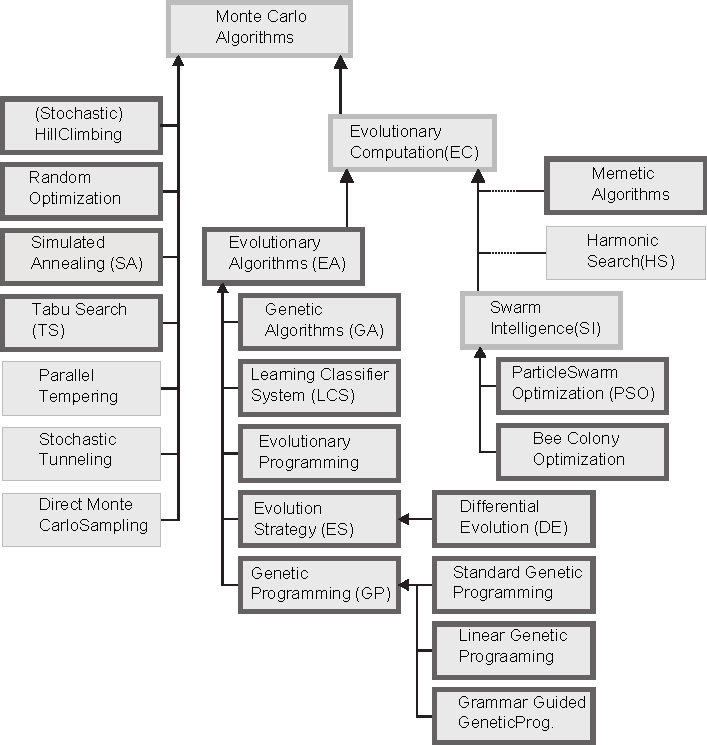
\includegraphics{Images/taxonomy_v2.pdf}


\newpage
\begin{thebibliography}{9}

\bibitem{weise}
  Thomas Weise,
  \emph{Global Optimization Algorithms, Theory and Application}.
  2nd Edition,
  2009
  http://it-weise.de.

\bibitem{hayes}
  Brian Hayes,
  \emph{A slight discrepancy}.
  http://bit-player.org/2011/a-slight-discrepancy
  http://devio.us/~tripzilch/raindrops/
  2011.
  
\bibitem{storn}
    Rainer Storn and Kenneth Price,
    \emph{Differential Evolution - A Simple and Efficent Heuristic for Global Optimization over Continous Spaces}.
    Journal of Global Optimization,
    1997
    
\bibitem{pygmo}
    Izzo, D.
    \emph{PyGMO and PyKEP: Open Source Tools for Massively Parallel Optimization in Astrodynamics}
    International Conference on Astrodynamics Tools and Techniques,
    2012. 

\bibitem{inspyred}    
    Aaron Lee Garrett
    \emph{inspyred: Bio-inspired Algorithms in Python}
    inspyred 1.0
    http://inspyred.github.com/
    2012
    
\bibitem{matlab-toolbox}
  Thomas Coleman, Mary Ann Branch and Andy Grace,
  \emph{Optimization Toolbox for use with Matlab User's Guide}
  Version 2,
  2002
  The Math Works, Inc.
  24 Prime Park Way, Natick, MA 01760-1500.
  
\bibitem{matlab-pso}
  M. Clerc, J. Kennedy
  \emph{"The particle swarm - explosion, stability, and convergence in a multidimensional complex space}
  Feb 2002
  Evolutionary Computation, IEEE Transactions on , vol.6, no.1, pp.58-73,
  doi: 10.1109/4235.985692

\bibitem{matlab-lus}
  M.E.H. Pedersen,
  \emph{Tuning \& Simplifying Heuristical Optimization}
  2010.  
  PhD Thesis
  University of Southampton

\end{thebibliography}


\end{document}